\documentclass[notitlepage]{hw}
\title{Jacobi Elliptic Functions in $\RR\times\RR$}
\date{}
\author{}

\begin{document}
\maketitle

\section{Introduction}

The Jacobi Elliptic functions come from non-elementary antiderivatives that arise when integrating
over an ellipse. We can define these functions in several ways. One such way is to define the
functions, $sn$, $cn$, and $dn$ as solutions to a system of ordinary differential equations.

\section{Jacobi Functions as solutions to ODEs}

We will begin by making a comparison of JEFs to Trig functions, with which we are familiar. Consider
$\sin{t}$ and $\cos{t}$. There are many definitions of these two functions, but we will consider a
definition that relates the two functions to ODEs, namely the system
\[
\begin{cases}
\dot{x}=y\\
\dot{y}=-x
\end{cases}.
\]
Under certain initial conditions, this leads to a basis composed of $\sin{t}$ and $\cos{t}$. It is with
this analogy that we can consider the JEFs.

Suppose we have a system of ODEs as follows
\[
\begin{cases}
\dot{x}=yz\\
\dot{y}=-zx\\
\dot{z}=-k^{2}xy
\end{cases}.
\]
These may seem like arbitrary selections for the system, but, as we will see, they are not. We need
to define $k$ before continuing; it is known as the modulus. On an ellipse, the value of $k$ is given
by
\[
k=\sqrt{1-{a^{2}\over b^{2}}},
\]
where $a$ is the major axis and $b$ is the semi-major axis.
We can also define $\kappa=\sqrt{1-k^{2}}$, known as the complimentary modulus. If we return to
our system, we can define the JEFs as solutions to the system under the following initial conditions:
\[
\begin{cases}
sn(0,k)=x(0)=0\\
cn(0,k)=y(0)=1\\
dn(0,k)=z(0)=1\\
\end{cases}.
\]

We can draw a relationship between $x$, $y$, and $z$ by forming a basis, much like we did with the
ODE definitions for $\sin{t}$ and $\cos{t}$. Namely, we have that
\[
\{ x,y,z \}\to\{ sn(t,k),cn(t,k),dn(t,k) \}.
\]
This gives rise to the immediate result that
\[
\begin{dcases*}
{d\over\dt}sn(t,k)=cn(t,k)dn(t,k)\\
{d\over\dt}cn(t,k)=-dn(t,k)sn(t,k)\\
{d\over\dt}dn(t,k)=-k^{2}sn(t,k)cn(t,k)
\end{dcases*}.
\]

With these properties in mind, we will consider a slightly more geometric view of JEFs.

\section{Jacobi Functions in a Geometric Sense}

We will begin our discussion by considering an ellipse centered about the origin in the cartesian plane.
Such an ellipse can be given by the equation
\[
\left({x^{2}\over a^{2}}\right) + \left({y^{2}\over b^{2}}\right) = 1.
\]
It will benefit us to consider the case where $b=1$, which gives the equation
\[
\left({x^{2}\over a^{2}}\right) + \left(y^{2}\right) = 1.
\]
We can take a given radius $r$ at the point $Q$ on the ellipse, and a given point $P$ at $a$. In
addition, we can call the angle between the the $x$ axis and the radius $\theta$. Rather than consider
a point $(x,y)$, we will actually consider a point $Q=(x(u),y(u))$, where $u$ is a function that we will
define later. We can define the JEFs in terms of this ellipse; we have

\vspace{0.5cm}

\begin{minipage}{0.5\textwidth}
\[
\begin{dcases*}
cn(u,k)=y\vphantom{\frac{0}{0}}\\
sn(u,k)={x\over a}\\
dn(u,k)={r\over a}
\end{dcases*}
\]
\end{minipage}
\begin{minipage}{0.5\textwidth}
\begin{center}
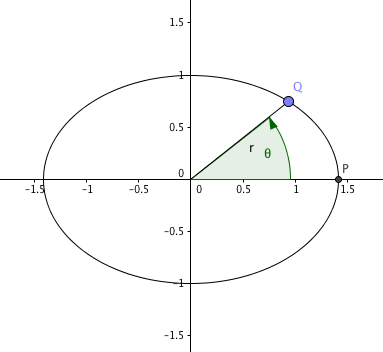
\includegraphics[scale=0.5]{ellipsis}\\

A generalized ellipse
\end{center}
\end{minipage}

\vspace{0.5cm}

We can establish some useful identities from this relationship, such as
\[
sn^{2}(u,k)+cn^{2}(u,k)=\left({x\over a}\right)^{2}+y^{2} = 1.
\]
This is similar to our trig identity of $\sin^{2}{x}+\cos^{2}{x}=1$. We also have that
\[
k^{2}sn^{2}(u,k)+dn^{2}(u,k)=1,
\]
which may not be as familiar, but it still holds true. Interestingly enough, we can formulate the
special (or maybe not so special) system of ODEs from the previous section using this new definition.

\section{Properties of Jacobi Functions}

Before we continue, we will want to outline some fundamental properties of the JEFs. Recall that we
already saw the analog to $\sin^{2}{x} + \cos^{2}{x} = 1$, which is
\begin{gather}
sn^{2}(u,k)+cn^{2}(u,k)= 1.
\end{gather}
In addition, we have
\begin{gather}
k^{2}sn^{2}(u,k)+dn^{2}(u,k)=1.
\end{gather}
We can also related the derivatives of the JEFs by
\begin{align}
{d\over\dt}sn(t,k)&=cn(t,k)dn(t,k)\\
{d\over\dt}cn(t,k)&=-dn(t,k)sn(t,k)\\
{d\over\dt}dn(t,k)&=-k^{2}sn(t,k)cn(t,k).
\end{align}
Since the functions are differentiable, we can talk about the limits of JEFs. If we let $k\to0$, we
can see that our defining system of ODEs becomes
\[
\begin{cases}
\dot{x}=yz\\
\dot{y}=-zx\\
\dot{z}=0
\end{cases},
\]
which yields a basis of $\{\sin{t},\cos{t},1\}$, implying that
\begin{align}
\lim_{k\to0^{+}}sn(t,k)&=\sin{t}\\
\lim_{k\to0^{+}}cn(t,k)&=\cos{t}\\
\lim_{k\to0^{+}}dn(t,k)&=1.
\end{align}
We can also see what happens a $k\to1$:
\begin{align}
\lim_{k\to1^{-}}sn(t,k)&=\tanh{t}\\
\lim_{k\to1^{-}}cn(t,k)&=\sech{t}\\
\lim_{k\to1^{-}}dn(t,k)&=\sech{t}.
\end{align}
These are enough

\section{Jacobi Functions as an Integral}

There is a third definition of JEFs that we can consider; the form they take from an integral. As we
saw previously, JEFs served as solutions to the system
\[
\begin{cases}
\dot{x}=yz\\
\dot{y}=-zx\\
\dot{z}=-k^{2}xy
\end{cases},
\]
but this is not the only system for which JEFs provide a solution. Consider the following system
\[
\begin{cases}
\dot{x}^{2}=(1-x^{2})(1-k^{2}x^{2})\\
\dot{y}^{2}=(1-y^{2})(\kappa^{2}+k^{2}y^{2})\\
\dot{z}^{2}=(1-z^{2})(z^{2}-\kappa^{2})
\end{cases}.
\]
We can transform the first ODE into
\[
{\dx\over\dt}=\sqrt{(1-x^{2})(1-k^{2}x^{2})},
\]
which is a separable equation. We can rewrite this as
\[
\int{\dx\over\sqrt{(1-x^{2})(1-k^{2}x^{2})}}=t,
\]
Which we may notice as an Elliptic Integral of the first kind. If we make the substitution
$x=\sin{u}$, then we have
\[
\int{\du\over\sqrt{1-k^{2}\sin^{2}{u}}}.
\]
This integral is not solvable by elementary means; rather we define the solution to be dependent on
$sn(u,k)$. There are similar integral definitions corresponding to $cn(u,k)$ and $dn(u,k)$.

\section{Applications to Elliptic Integrals}

We saw previously that we cannot integrate
\[
\int{\dt\over\sqrt{1-k^{2}\sin^{2}{t}}}
\]
using elementary methods. We saw that this integral came from a substitution on
\[
\int{\dx\over\sqrt{(1-x^{2})(1-k^{2}x^{2})}}.
\]
Recall that by property $(3)$, we have
\[
{d\over\dt}sn(t,k)=cn(t,k)dn(t,k)=\sqrt{(1-sn^{2}(t,k))(1-k^{2}sn^{2}(t,k))}
\]
by property $(1)$. This leads us to the result that
\[
\int{d\over\dt}sn(t,k)=sn(t,k)=\int\sqrt{(1-sn^{2}(t,k))(1-k^{2}sn^{2}(t,k))}\dt.
\]
Note that we can invert the $sn(t,k)$, which leads us to
\[
sn^{-1}(t,k)=\int{\dt\over\sqrt{(1-t^{2})(1-k^{2}t^{2})}}.
\]
We can similarly formulate definitions for $cn^{-1}(t,k)$ and $dn^{-1}(t,k)$.
\end{document}
